\documentclass[10pt]{beamer} %handout in[10pt, handout]
\usepackage[round]{natbib}
\newcommand{\ud}{\,\mathrm{d}}
\newcommand{\vx}{\mathbf{x}}
\usetheme{Copenhagen}
\setbeamertemplate{navigation symbols}{}

\title{Causal Bayesian network exploration of \\ the UK Biobnak data}
\subtitle{Week 4 Report}
\author[The Biobank Group]{The Biobank Group}
\institute[ATI]{The Alan Turing Institute}
\date{July 15, 2016}
\begin{document}

%----------- titlepage ----------------------------------------------%
\begin{frame}[plain]
  \titlepage
\end{frame}
%----------- slide --------------------------------------------------%
\begin{frame}[plain]{Overview}
 \frametitle{The UK Biobank Project}
    \tableofcontents
\end{frame}
%----------- Section --------------------------------------------------%
\section{Introduction}
\begin{frame}[plain]{Intro}

\end{frame}

%----------- slide --------------------------------------------------%
\section{Data Cleaning}
\begin{frame}[plain]{Data Cleaning}

\end{frame}


%----------- Section --------------------------------------------------%
\section{Dimention Reduction}
\begin{frame}[plain]{Dimention reduction}

\end{frame}

%----------- slide --------------------------------------------------%
%----------- Section --------------------------------------------------%
\section{Prelimiary Causal Study}

\begin{frame}[plain]{Causal inference}
Graphical representation of causal relationships of variables.
\begin{figure}
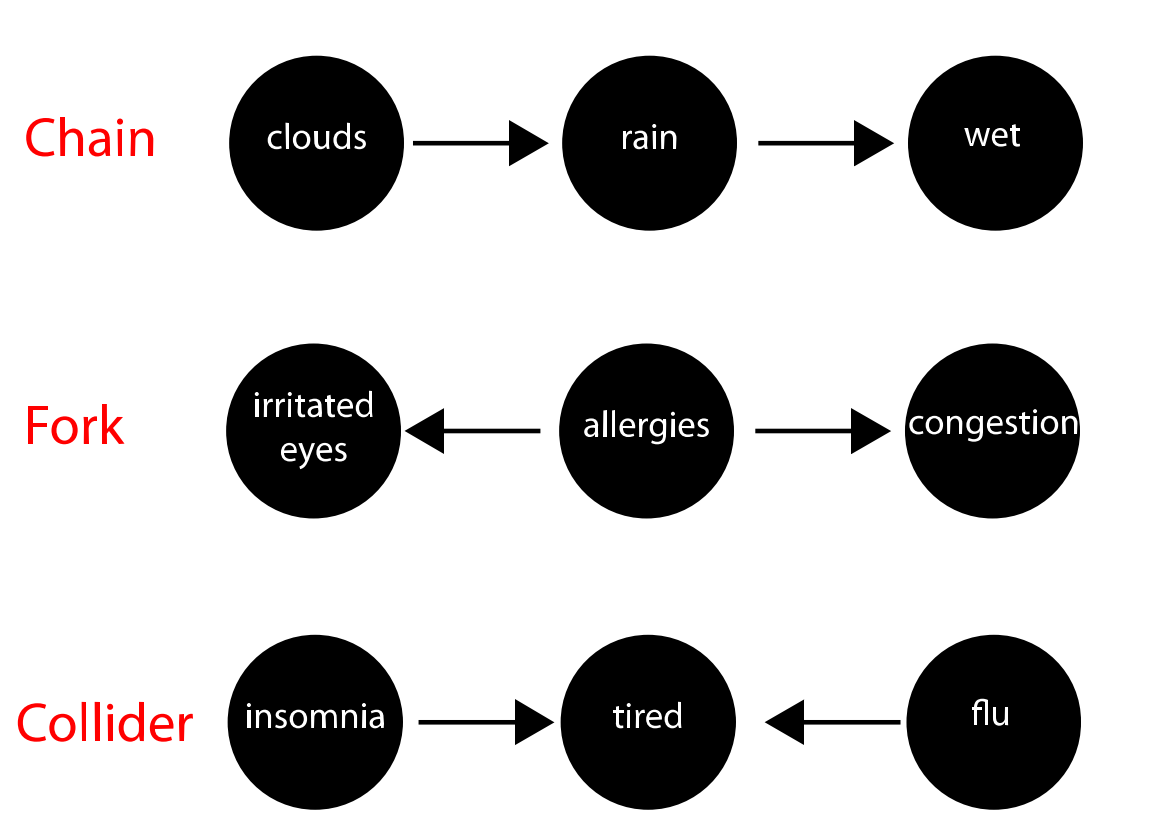
\includegraphics[width = 0.9\textwidth]{images/CIexample.png}
\end{figure}
\end{frame}

%----------- slide --------------------------------------------------%
\begin{frame}[plain]{Bayesian Network}

{\begin{block}{Bayesian Network}
Given a probability distribution $P$ on a set of variables $X$, a Bayesian Network for $(P,X)$ is
\begin{itemize}
\item a DAG (Directed Acyclic Graph) $G$
\item $G$ is a minimal Independence-map of $P$
\end{itemize}
\end{block}}

\begin{figure}
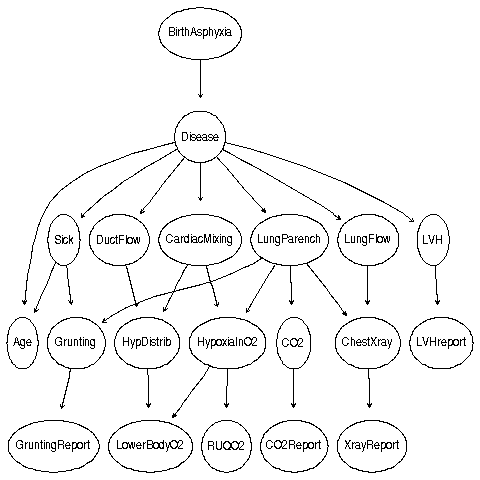
\includegraphics[width = 0.5\textwidth]{images/BNexample.png}
\end{figure}
\end{frame}

%----------- slide --------------------------------------------------%
\begin{frame}[plain]{Causal study using the Bayesian Networks}

\setbeamercovered{transparent}
\onslide<1->{\begin{block}{Causal study of the Biobank data}
\begin{itemize}
\item Represent the joint distribution of the variables by Bayesian networks.
\item Find possible causal relationship from the Bayesian networks.
\end{itemize}
\end{block}}

\onslide<2->{\begin{block}{Learning the Bayes Nets}
\begin{itemize}
\item Structure learning: search the possible graph representations
\begin{itemize}
\item Contraint-based algorithms: Independence tests:  PC
\item Score-based algorithms: greedy search algorithms based on  likelihood, BIC
\end{itemize}

\item Parameter learning
\begin{itemize}
\item More model assuptions and estimate the paramter by maximum likelihood estimation or Bayesian estimation. 
\end{itemize}
\end{itemize}
\end{block}}

\end{frame}

%----------- slide --------------------------------------------------%
\begin{frame}[plain]{A first search}
PC search on a set of hypothesis driven varialbes -- numerical variables.
\begin{figure}
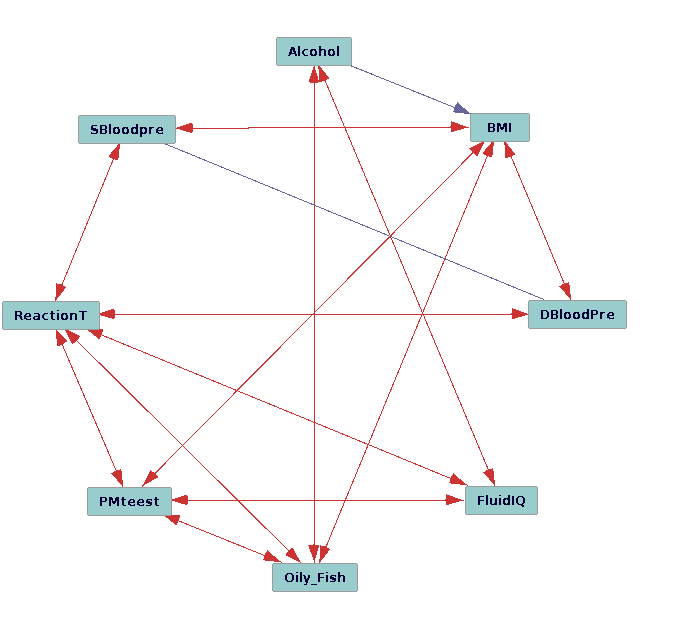
\includegraphics[width = 0.8\textwidth]{images/cont.png}
\end{figure}
\end{frame}

%----------- slide --------------------------------------------------%
\begin{frame}[plain]{A first search}
PC search on a set of hypothesis driven varialbes -- categorical variables.
\begin{figure}
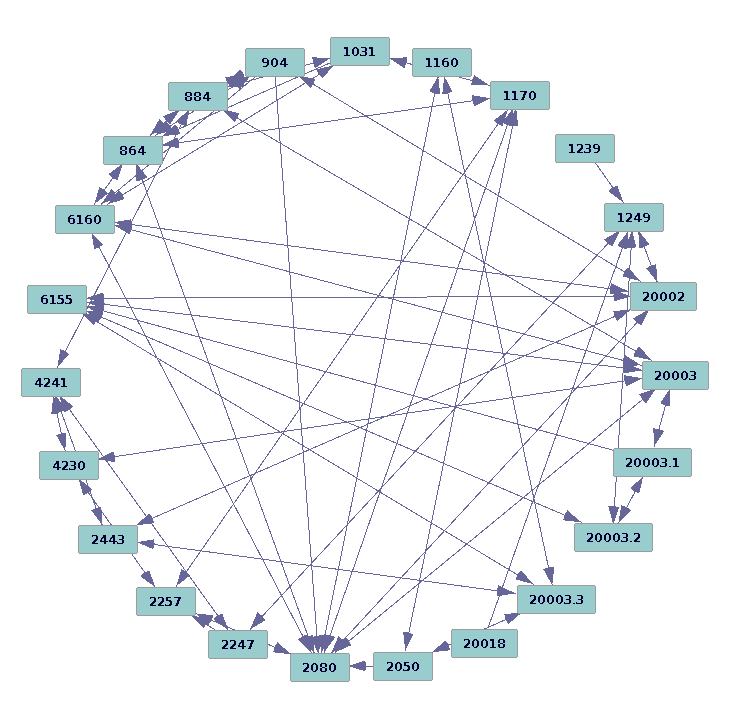
\includegraphics[width = 0.75\textwidth]{images/cat.png}
\end{figure}
\end{frame}

%----------- Section --------------------------------------------------%
%----------- slide --------------------------------------------------%
\section{Next Step}
\begin{frame}[plain]{Next Step}

\end{frame}


\end{document}
